%!TEX root = ./thesis-main.tex
\chapter{Design}
\section{Layout dell'interfaccia} \label{section:interface-layout}
Il layout dell'interfaccia grafica è stato pensato per rappresentare nel modo più semplice ed intuitivo l'ambiente della simulazione.  La figura \ref{fig:interface-layout} rappresenta un mockup utilizzato durante la fase di progettazione dell'interfaccia. Si possono individuare le seguenti sezioni:
\begin{itemize}
	\item \textbf{Barra di navigazione}: nella parte alta dell'interfaccia è presente una barra di navigazione contenente il titolo e il pulsante per avviare o mettere in pausa la simulazione, ancorato all'estrema destra. Molte interfacce web moderne presentano questo tipo di elemento come \textit{header} della pagina web principale, inteso come punto centrale dal quale è possibile accedere a tutte le sezioni e funzionalità. Questo fornisce all'interfaccia un punto di espandibilità dell'applicativo, come l'aggiunta di una barra di ricerca o di un menù detto ad ``hamburger''. Sarebbe stato possibile, per esempio, inserire una barra di ricerca per i nodi, filtrandoli per categorie di proprietà. Questo tipo di funzionalità è indirizzato a lavori futuri (vedi \cref{item:research-bar}). 
	\item \textbf{Canvas grafico}: la sezione principale di questa interfaccia. All'interno di un contesto grafico bidimensionale vengono rappresentati i nodi della simulazione. Ogni nodo è rappresentato come un cerchio pieno, avente centro le coordinate del nodo e raggio un valore variabile che può essere impostato dall'utente nella sezione descritta successivamente. Lo spazio bidimensionale ha come sfondo una griglia, che  fornisce un riferimento visivo e un aiuto all'orientamento. Funzionalità non banale di questa sezione è che l'utente può spostare il contesto visivo trascinando il cursore sullo schermo, oltre che a effettuare un ingrandimento o una diminuzione della scala. Per ottenere questo tipo di comportamenti sono stati adottati meccanismi ad hoc per il calcolo dello spostamento del \textit{drag} e dello \textit{zoom-in}/\textit{zoom-out}. Infine, facendo click su un nodo è possibile selezionarlo, andando a riportare nella sezione di ispezione del nodo tutte le sue caratteristiche principali.
	\item \textbf{Informazioni e controlli sul canvas}: in questa sezione vengono raccolte le principali informazioni riguardo allo stato attuale del \textit{canvas}, come il fattore di \textit{zoom} corrente, la differenza di traslazione rispetto all'origine e la grandezza del raggio utilizzato per rappresentare i nodi. Il fattore di scala è riportato, oltre nella sua forma numerica anche tramite una barra di progresso, la cui lunghezza varia in base alla percentuale di zoom raggiunta rispetto al valore massimo. Altro oggetto con cui l'utente può interagire è uno \textit{slider}, al variare del quale viene aggiornato il raggio utilizzato per disegnare i nodi nel \textit{canvas}. I parametri legati al \textit{rendering} (fattore minimo e massimo di scala, altezza e larghezza del canvas, numero di iterazioni di scala etc.) sono raggruppati in un unico oggetto e quindi aperti a modifiche.
	\item \textbf{Sezione di ispezione di un nodo}\label{item:node-inspection}: qui vengono rappresentate tutte le informazioni riguardanti un nodo. Sono presenti quindi il codice identificativo, la posizione nello spazio bidimensionale, proprietà, i contenuti (intesi come una lista di molecole alle quali vengono associate le relative concentrazioni), e le reazioni (Vedi \ref{item:reactions}). Per le ultime tre categorie sono stati usati degli elementi grafici che possono essere espansi o ``collassati'' in quanto non è garantito che queste proprietà siano presenti (sempre per il fatto che Alchemist può rappresentare una certa gamma di simulazioni tra loro eterogenee).
\end{itemize}

\begin{figure}[htb]
	\centering
	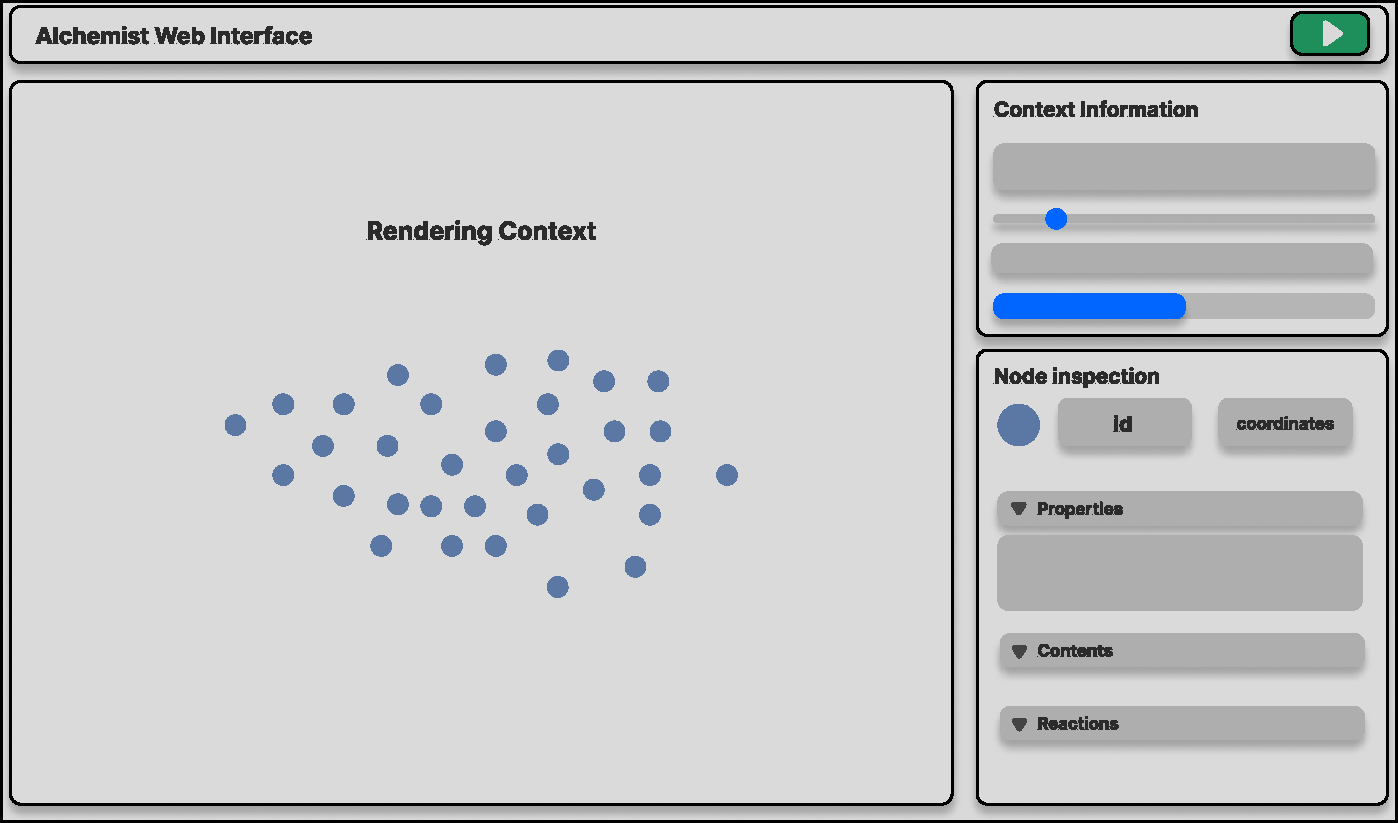
\includegraphics[scale=0.65]{imgs/Interface_Layout.pdf}
	\caption{Mockup dell'interfaccia grafica}
	\label{fig:interface-layout}
\end{figure}

\section{Connessione al server GraphQL}\label{section:graphql-connection}
In questa sezione viene esplorato come l'interfaccia web interagisce con le \ac{API} GraphQL per effettuare operazioni sul server e impiegare successivamente i risultati di tali operazioni per mostrarli graficamente. Nella figura \ref{fig:general-client-architecture-graphics} vengono mostrate le principali componenti protagoniste di questo meccanismo. Le descriviamo in questo modo:

\begin{itemize}
	\item \textbf{Client Application}: questo \textit{package} contiene tutte le componenti grafiche che vengono rappresentate all'interno della pagina principale. Ogni componente, una volta che l'applicativo viene avviato, è tradotto al browser in formato HTML.
	\item \textbf{ClientConnection}: punto di accesso attraverso il quale è possibile effettuare tutte le operazioni definite secondo lo \textit{schema} GraphQL. All'interno di questo oggetto è dichiarata l'unica istanza per l'intero progetto che funge da punto di accesso per le operazioni sul server secondo lo schema definito. 
	\item \textbf{SimulationControlApi}: questo oggetto contiene tutte le funzioni necessarie a controllare lo stato della simulazione e dipende strettamente dalla componente \textbf{ClientConnection}. Si parla quindi di funzioni utili all'avvio, alla sospensione e terminazione della simulazione. Notare come queste siano tutte operazioni di tipo \textit{mutation}.
	\item \textbf{EnvironmentApi}: è l'oggetto utile a recuperare le informazioni riguardanti un nodo, lo stato \textit{attuale} dell'\textit{Environment}, ma soprattutto utile a recuperare la posizione dei nodi in tempo reale, quindi attraverso l'utilizzo di una \textit{subscription}. 
	\item \textbf{GeneratedSources}\label{item:generated-sources}: questo pacchetto contiene tutte le risorse generate a partire dallo schema GraphQL esposto dal server. È utilizzato dagli oggetti \textbf{EnvironmentApi} e \textbf{SimulationControlApi} nell'utilizzo dei tipi di dato corretto durante la composizione delle operazioni sul server.
\end{itemize}

\begin{figure}[htb]
	\centering
	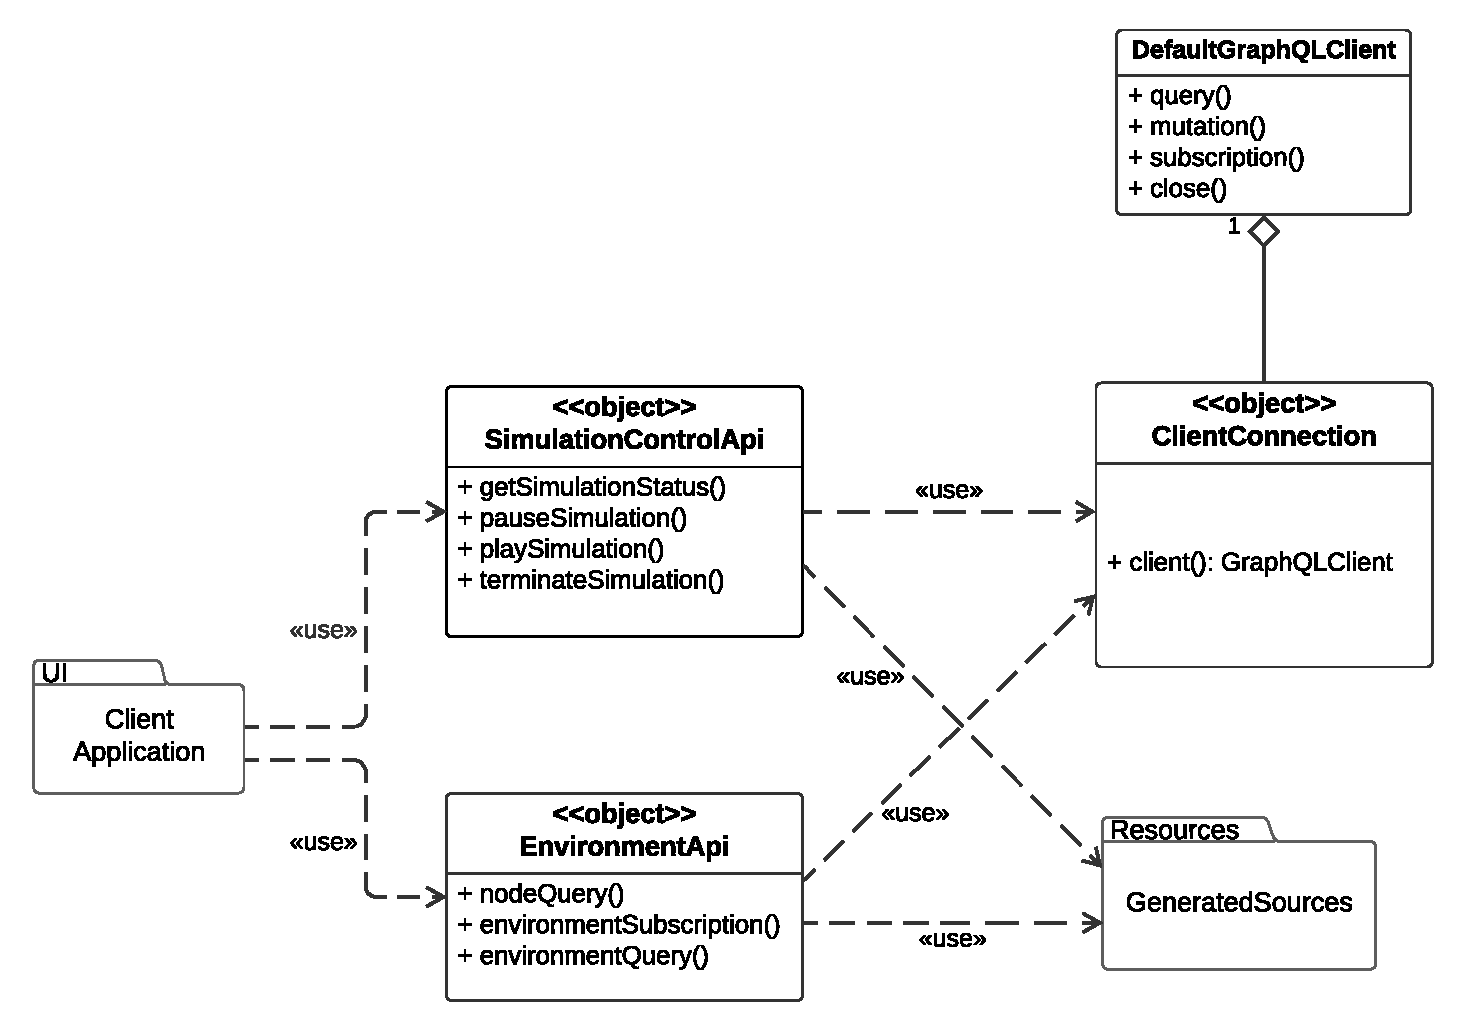
\includegraphics[scale=0.52]{imgs/General_Architecture_Web_Client.pdf}
	\caption{Utilizzo della connessione al client GraphQL}
	\label{fig:general-client-architecture-graphics}
\end{figure}

Gli oggetti \textbf{SimulationControlApi} e \textbf{EnvironmentApi} sono stati implementati attraverso il design pattern \textit{Singleton}~\cite{Gamma1994}. Sebbene quest'ultimo, se abusato o implementato in modo non adeguato sia considerato di fatto un ``anti-pattern'' \footnote{\url{https://code.google.com/archive/p/google-singleton-detector/wikis/WhySingletonsAreControversial.wiki}}, in questa situazione risulta essere molto comodo, specialmente considerando la necessità di un unico punto di accesso comune al client che effettua le query sul server. Risulterebbe infatti inutile, per ogni componente grafico che ne necessita, istanziare un altro client GraphQL dal quale effettuare query. Lo stesso vale anche nell'ipotesi in cui vengano utilizzate delle proprietà che fungono da parametri di configurazione dell'applicativo. Un \textit{Singleton} può fornire un punto centralizzato per queste impostazioni.

\section{Architettura generale client web}\label{section:client-web-architecture}
Il diagramma UML in figura mostra la soluzione adottata alla necessità di ospitare la pagina web finale all'interno di un browser web. Dallo schema in \cref{fig:client-web-structure-graphics} è possibile individuare le seguenti sezioni:

\begin{itemize}
	\item \textbf{OutputMonitor}: interfaccia di Alchemist che fornisce un modo flessibile per osservare la progressione delle simulazioni tramite l'esposizione di \textit{hook standard}.  Quest'ultimi si riferiscono a punti predefiniti all'interno del ciclo di vita della simulazione (avvio della simulazione, fine di ogni passo della simulazione, fine della simulazione) ai quali è possibile collegare meccanismi personalizzati. Questa interfaccia aderisce al design pattern \textit{Observer}~\cite{Gamma1994}.
	\item \textbf{GraphQLServer}: implementazione dell'interfaccia  \texttt{OutputMonitor}. Questa classe avvia il server GraphQL all'avvio della simulazione e si assicura che al termine della simulazione il server venga chiuso.
    \item \textbf{WebUIMonitor}: estensione della classe \texttt{GraphQLServer}, che avvia il server sul quale viene presentata la pagina web contenente l'interfaccia grafica esplorata in sezione \ref{section:interface-layout}. Come per la classe da cui eredita, al momento della terminazione della simulazione, il server viene chiuso. L'estensione alla classe \texttt{GraphQLServer} permette che la simulazione venga configurata con \texttt{WebUIMonitor} come \texttt{OutputMonitor}, avviando contemporaneamente il server GraphQL e il server che ospita la pagina web che rappresenta l'interfaccia grafica.
    In questo contesto, è necessario configurare una nuova \textit{route} nel server per caricare la pagina principale \texttt{index.html}. Per semplificare il processo, questa \textit{route} verrà mappata per rispondere alle richieste GET alla radice (``\texttt{/}'') servendo la risorsa \texttt{index.html}. Ciò consente ai client di accedere direttamente alla pagina specificando l'indirizzo e la porta del server.
	\item \textbf{Generated Artifacts}: questo pacchetto include tutti i file necessari alla composizione di un unico file di output, con estensione \texttt{.js} (processo noto anche come \textit{bundling}). Il file che ne risulterà verrà servito al server in modo statico. Il server può essere configurato per andare a recuperare tutti gli artefatti necessari al \textit{bundling} a partire da un percorso remoto specificato. Ciò significa che nel caso fossero stati dichiarati dei file CSS o JavaScript separati, questi sarebbero stati comunque coinvolti nella generazione del file di output e sarebbero stati accessibili tramite \ac{URL} che iniziano dal percorso remoto (in questo caso ``\texttt{/}'').	
	Ad esempio, se il pacchetto base contiene un file chiamato ``\texttt{styles.css}" e il percorso remoto è ``\texttt{/static}", il file ``\texttt{styles.css}" può essere accessibile all'URL ``\texttt{static/styles.css}" nell'applicazione. 
	
\end{itemize}

\begin{figure}[htb]
	\centering
	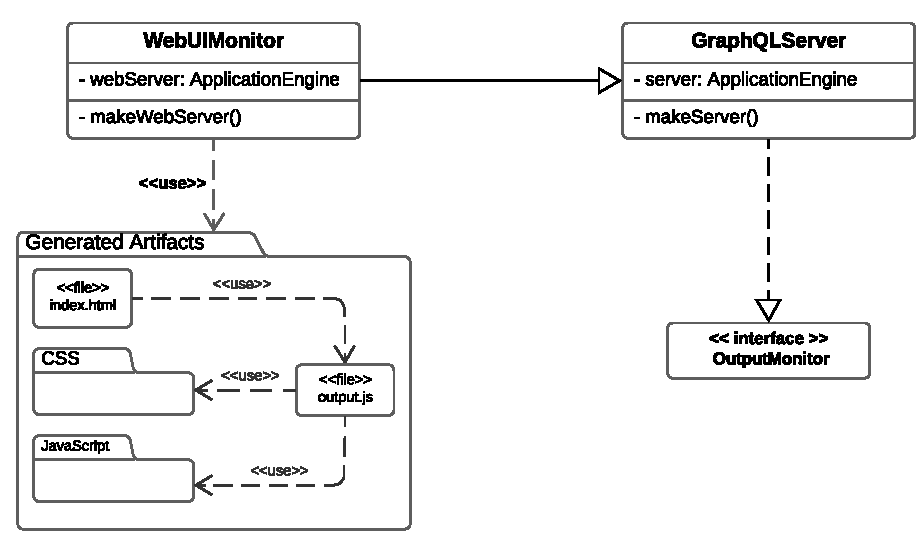
\includegraphics[scale=0.7]{imgs/Web_Client_Structure.pdf}
	\caption{Architettura generale del client web}
	\label{fig:client-web-structure-graphics}
\end{figure}

\section{Struttura della pagina web} \label{section:page-structure}
Si vuole definire ora la struttura della pagina che si presenterà nel momento in cui gli utenti si collegheranno al client web. La struttura finale si presenta come una gerarchia di componenti grafiche. Ogni componente è raggruppata all'interno di contenitori logici per una gestione efficiente e una navigazione chiara dell'interfaccia. Questo è ottenuto attraverso l'utilizzo di oggetti che dispongono i componenti figli secondo un layout prestabilito. Sono stati creati contenitori modulari e riutilizzabili per facilitare lo sviluppo e la manutenzione dell'interfaccia, oltre che a fornire un punto di scalabilità. Di conseguenza, ciò consente di comporre e combinare diverse componenti per soddisfare le esigenze specifiche delle diverse sezioni dell'applicazione. La figura \ref{fig:page-structure} descrive la suddetta struttura.

\begin{figure}[htb]
	\centering
	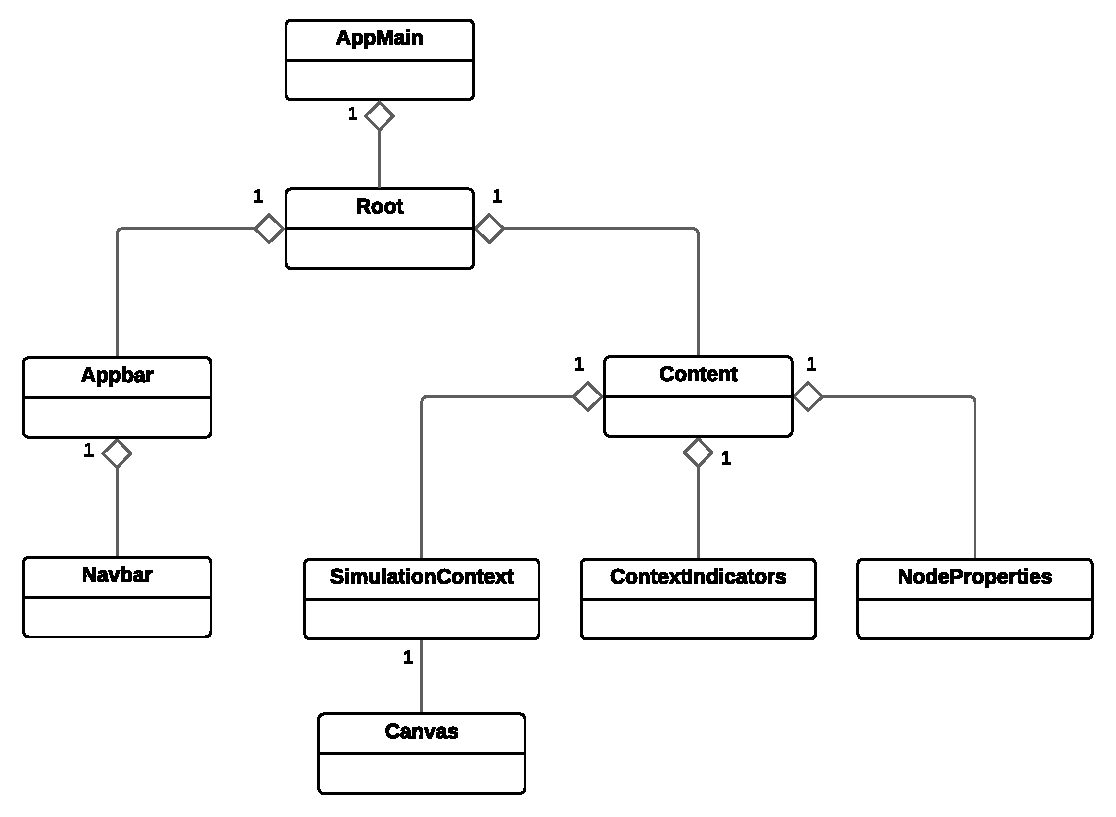
\includegraphics[scale=0.82]{imgs/Struttura pagina web.pdf}
	\caption{Diagramm UML delle classi per le componenti della pagina web}
	\label{fig:page-structure}
\end{figure}

L'applicazione ha inizio nella classe classe \texttt{AppMain} che effettua una query sul \ac{DOM} per la ricerca dell'elemento padre con identificativo ``root''. Una volta ottenuto, vengono aggiunti, come componenti figli, le classi \texttt{Appbar} e \texttt{Content}, che, rispettivamente, danno forma alla barra di navigazione e alla parte corposa della pagina (il contenuto principale). In particolare per quest'ultimo, si può osservare l'esistenza di una corrispondenza uno a uno tra le sezioni descritte in \ref{section:interface-layout}: 
\begin{itemize}
	\item \texttt{SimulationContext}: classe padre contenente il canvas di disegno.
	\item \texttt{ContextIndicators}: contiene tutte le singole entità grafiche che provvedono a dare informazioni riguardo al canvas.
	\item \texttt{NodeProperties}: fornisce in un layout riassuntivo, le principali informazioni riguardanti un nodo selezionato dal canvas.
\end{itemize}
Come per gli elementi appena citati, è importante sottolineare la correlazione tra i macro-elementi che hanno un ruolo all'interno dell'interfaccia utente e le classi principali che compongono la struttura finale della pagina HTML. Il mantenimento di questa relazione biunivoca è di aiuto allo sviluppatore e mantiene ordinato e scalabile il codice sorgente.


